\documentclass{article}
\usepackage[utf8]{inputenc}
\usepackage{hyperref}
\usepackage{csquotes}
\usepackage{graphicx}

\graphicspath{ {res/} }
\renewcommand{\familydefault}{\sfdefault}
\hypersetup{
    colorlinks=true,
    linkcolor=none,
    urlcolor=magenta,
}

\title{XYZ Image Specification (XYZ)}
\author{Chika Games}
\date{January 2020}

\begin{document}

\maketitle
\tableofcontents

\newpage

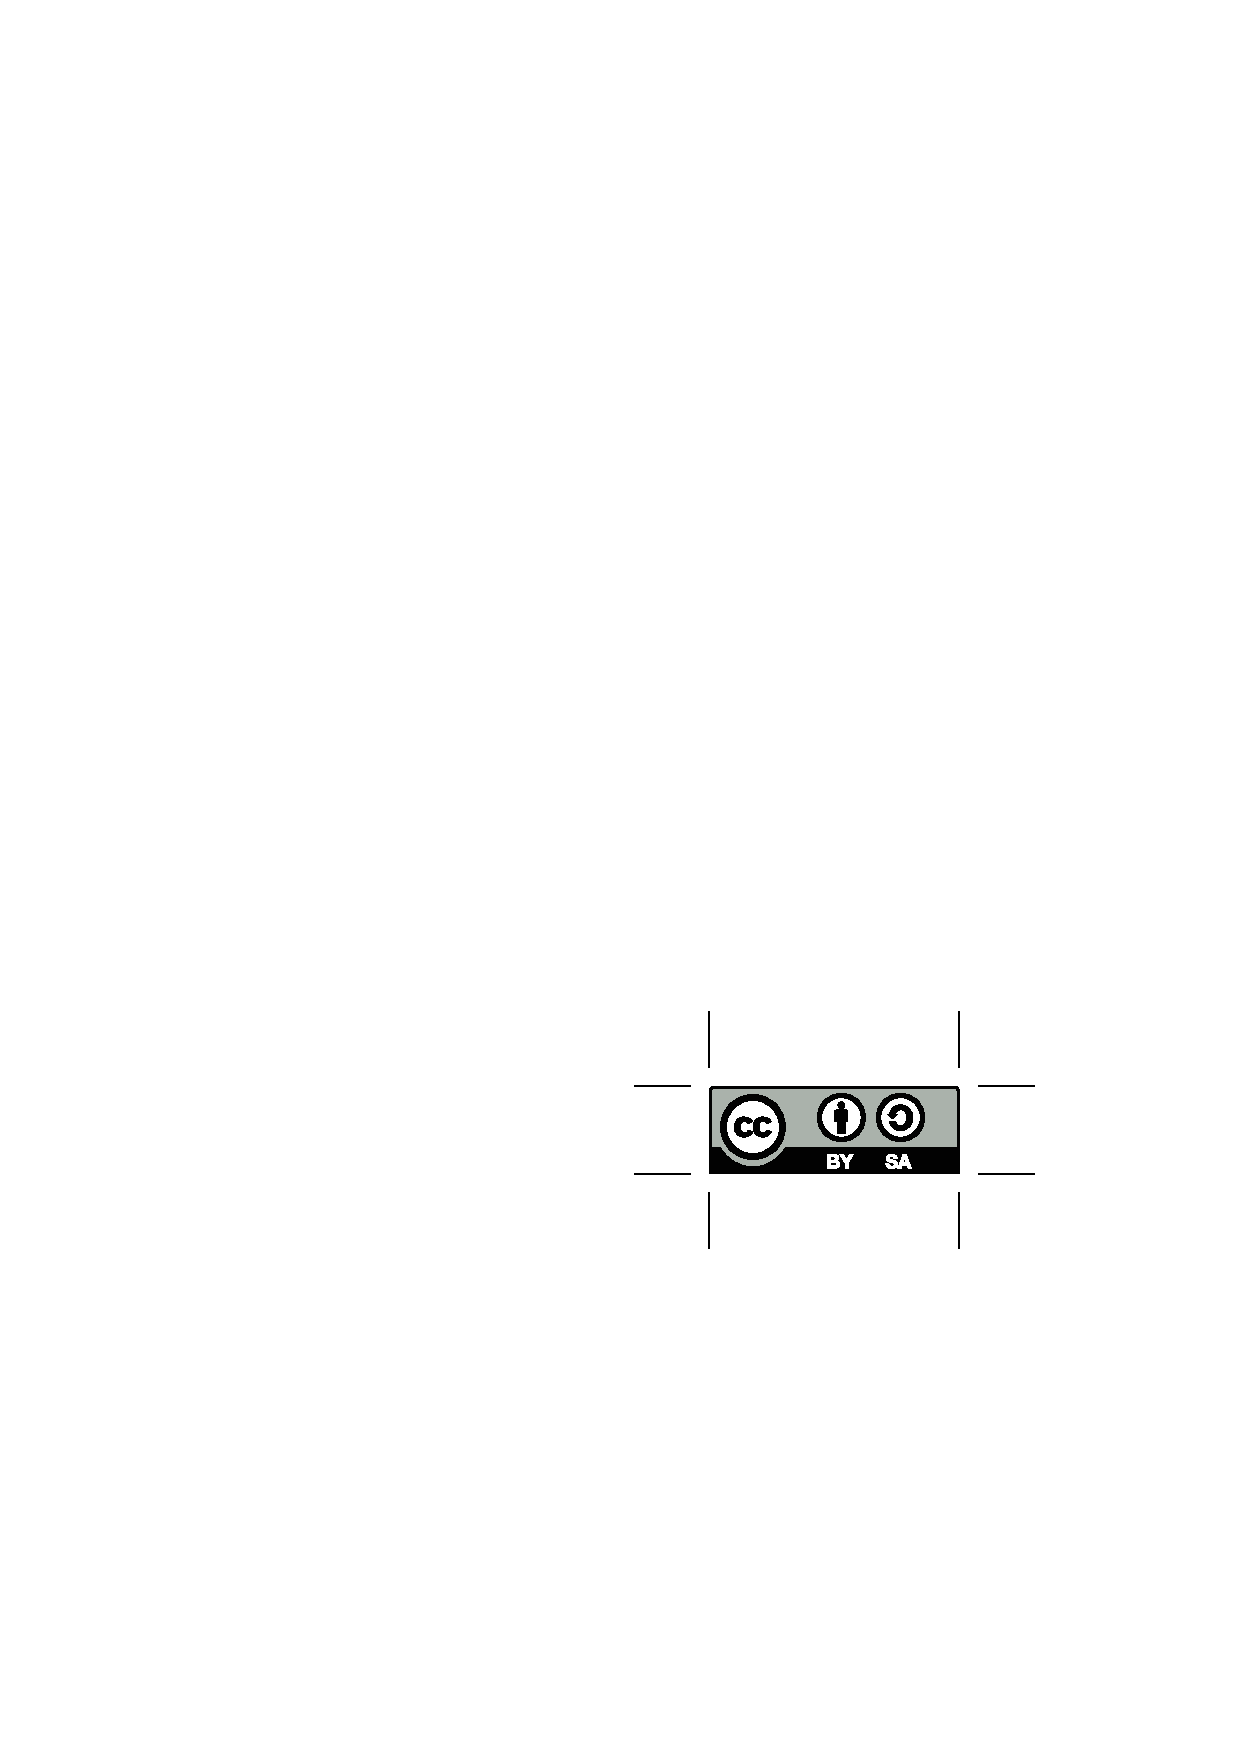
\includegraphics[scale=0.75]{by-sa}

This work is licensed under the Creative Commons Attribution-ShareAlike 4.0 International License. To view a copy of this license, visit \url{http://creativecommons.org/licenses/by-sa/4.0/} or send a letter to Creative Commons, PO Box 1866, Mountain View, CA 94042, USA. Copyright \copyright~2019-\the\year~Chika Games.

The RPG Maker trademark and copyright are property of Enterbrain, Inc. and Kadokawa Corporation. All rights belong to their respective owners.

\newpage

\section{Introduction}
The XYZ file format (\textit{.xyz}) is a custom image format used by RPG Maker 2000 and 2003. This format is palette-based and stores three 8-bit color channels (red, green, and blue) for a total of 24 bits per pixel. This results is a design that is simple to read and write.

This specification is part of a larger collection that can be found at the following URL: \url{https://github.com/chika-games/RPG-Maker-Specifications}.

\section{Data Types}
This section describes the various data types that will be used throughout this specification.

Little-endian byte order is assumed for all types; the least significant byte is stored first, and the most significant byte is stored last.

Types may be appended with \textit{[n]} in order to denote a contiguous array of the type where \textit{n} is the number of elements. For example, \textit{U8[4]} denotes an array of four unsigned 8-bit integers.

\subsection{Basic Data Types}
These types are considered \textit{primitive} as all other data types are constructed using these:

\begin{table}[h!]
\centering
\begin{tabular}{|l|l|}
\hline
\textbf{Type} & \textbf{Description}        \\ \hline
U8            & An unsigned 8-bit integer.  \\ \hline
U16           & An unsigned 16-bit integer. \\ \hline
\end{tabular}
\end{table}

\subsection{Compound Data Types}
These types are constructed using a combination of basic data types.

\subsubsection{RGB Type}
The \textit{RGB} type represents a color with three color channels: red, green, and blue.

\begin{table}[h!]
\centering
\begin{tabular}{|l|l|l|}
\hline
\textbf{Field} & \textbf{Type} & \textbf{Description}          \\ \hline
Red            & \textit{U8}   & The red-value of the color.   \\ \hline
Green          & \textit{U8}   & The green-value of the color. \\ \hline
Blue           & \textit{U8}   & The blue-value of the color.  \\ \hline
\end{tabular}
\end{table}

\section{XYZ File Structure}
This section details the overall structure of an XYZ file.

\begin{table}[h!]
\centering
\begin{tabular}{|l|l|l|}
\hline
\textbf{Field} & \textbf{Type}                   & \textbf{Description}                                     \\ \hline
Signature      & \textit{U8}                     & The file's signature. Should always be \textquote{XYZ1}. \\ \hline
Width          & \textit{U8}                     & The image's width in pixels.                             \\ \hline
Height         & \textit{U8}                     & The image's height in pixels.                            \\ \hline
Palette        & \textit{RGB[256]}               & The image's color palette.                               \\ \hline
PixelData      & \textit{U8[Width \cdot Height]} & The image's pixel data.                                  \\ \hline
\end{tabular}
\end{table}

\textbf{Note:} The \textit{Palette} and \textit{PixelData} fields are compressed using the \href{https://en.wikipedia.org/wiki/DEFLATE}{DEFLATE} compression algorithm; all data after the first 8 bytes must be decompressed before use.

\end{document}
